\section{Resultados}

\subsection{Análisis con cantidad de términos variable}

\subsubsection{Comparación del error absoluto en función de la entrada, para varias cantidades de términos fijas}


En los primeros gráficos comparamos los errores absolutos al hacer $|f(x)-cos(x)|$, usando la función $cos(x)$ de C$++$, para diferentes cantidades de términos T. En primer lugar, graficamos con T tomando valores entre 2 y 5, para $x$ entre 0 y 3 evaluando en intervalos de 0.2

\begin{center}
	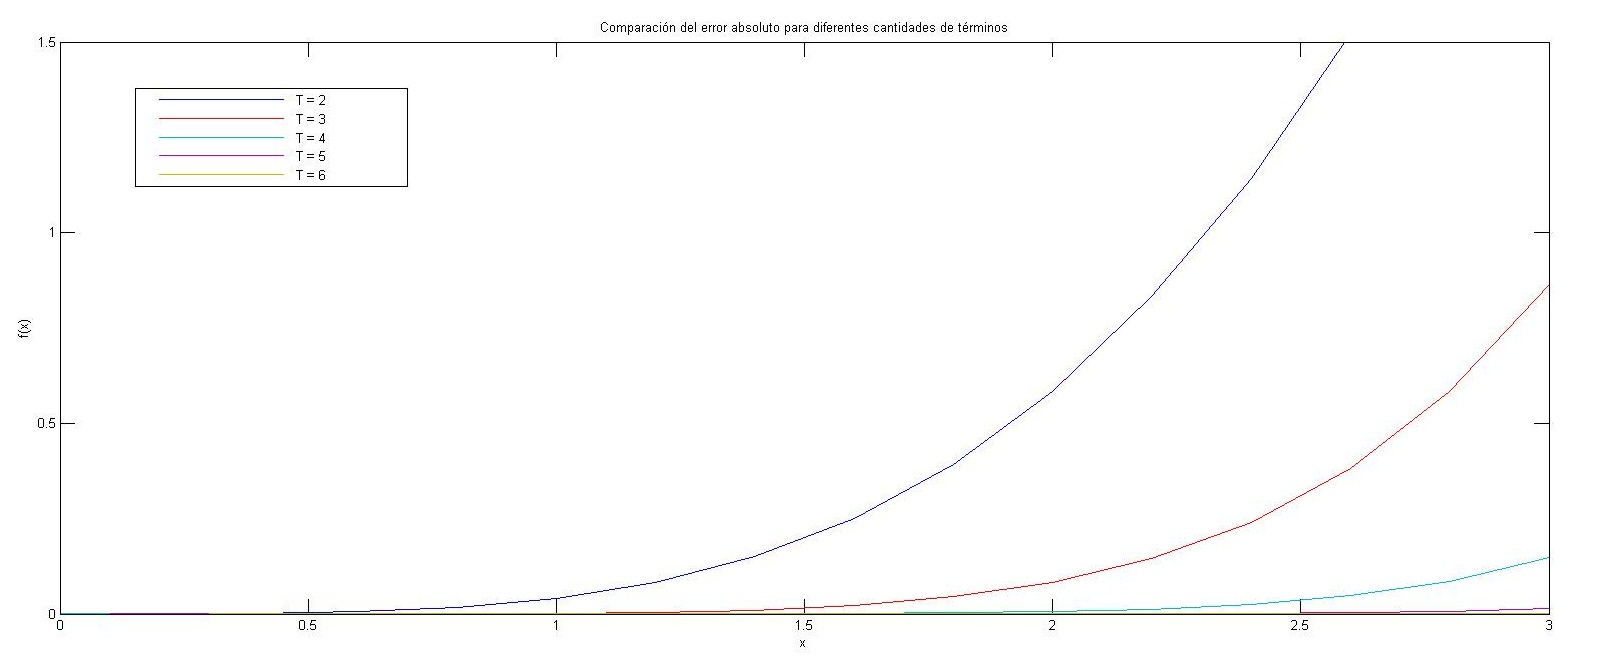
\includegraphics[scale=0.45]{../img/2a-T2:5.jpg} \\
 	\scriptsize{\textsf{\textbf{Gr\'afico 1.1, comparación del error absoluto para diferentes cantidades de términos T de la serie}}}
 	
\end{center}

Luego hicimos el mismo gráfico pero para T con valores entre 6 y 8. Nótese que la escala en el eje $y$ está en todos casos multiplicada por $10^{-3}$.

\begin{center}
	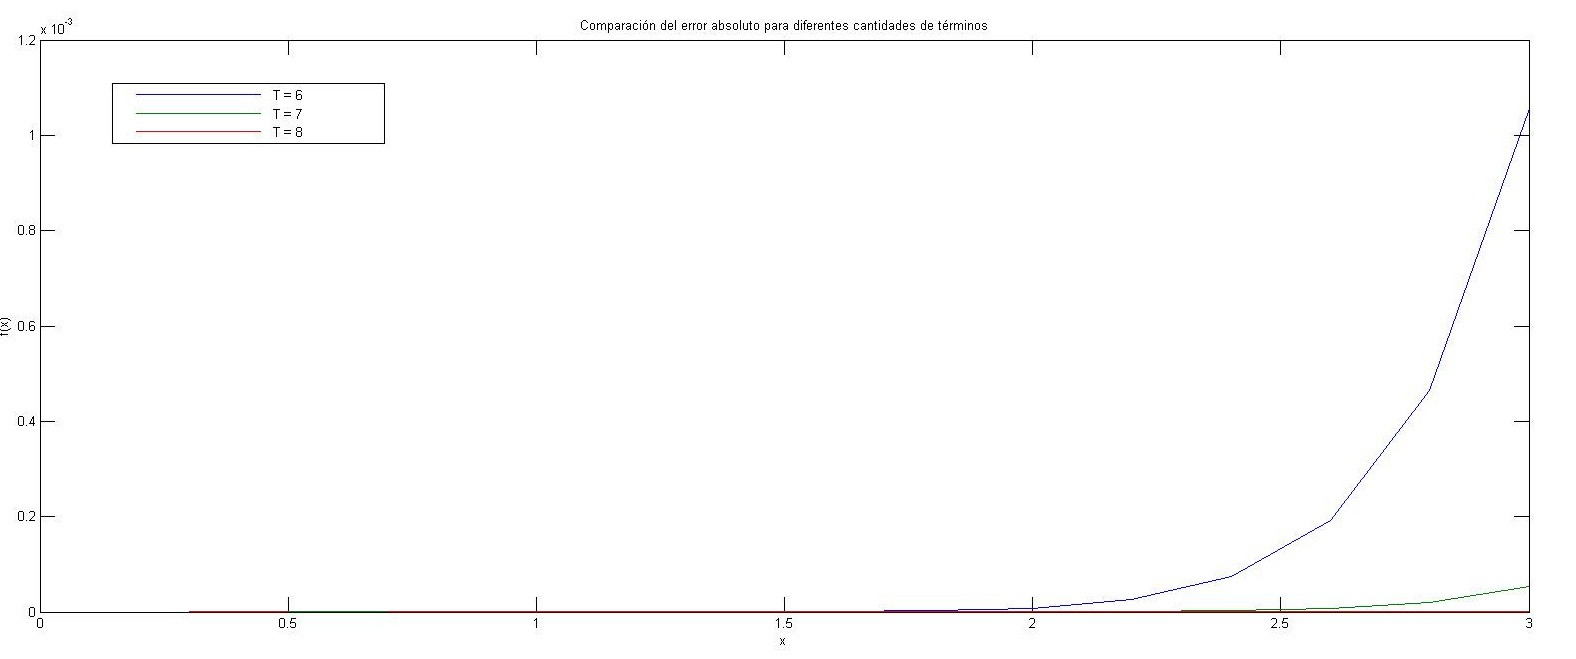
\includegraphics[scale=0.45]{../img/2a-T6:8.jpg} \\
 	\scriptsize{\textsf{\textbf{Gr\'afico 1.2, comparación del error absoluto para diferentes cantidades de términos T de la serie}}}
 	
\end{center}


\subsubsection{Gráficos del error en función de la cantidad de términos, para varias entradas fijas}

Una vez terminado de comparar diferentes T, nos interesó comparar el comportamiento del error para diferentes $x$, en función de T. Para esto, obtuvimos el cálculo de $f(x)$ para todas las cantidades de términos de 2 a 8, para diferentes $x$, y obtuvimos el error absoluto de la misma manera que antes.

\begin{center}
	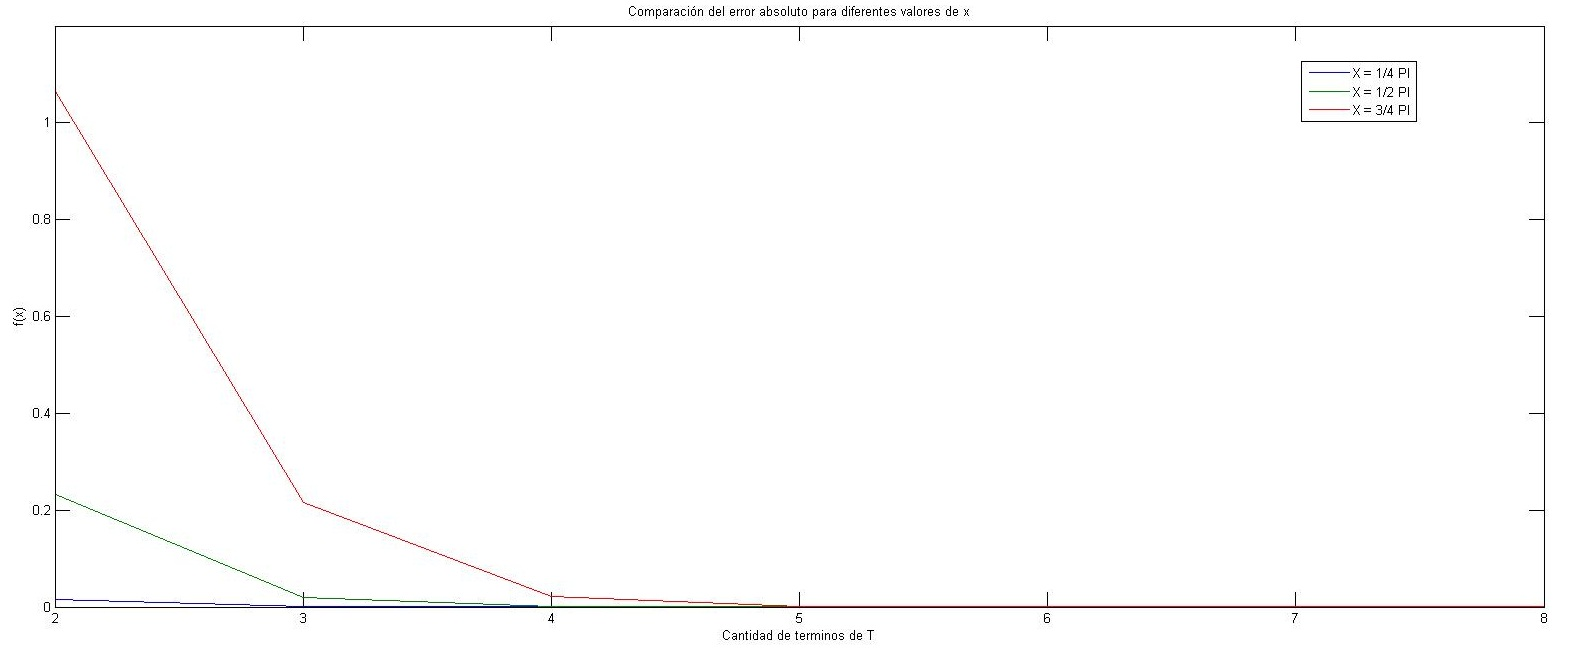
\includegraphics[scale=0.45]{../img/2a-xmenorPI.jpg} \\
 	\scriptsize{\textsf{\textbf{Gr\'afico 2.1, comparación del error absoluto para diferentes entradas $x$}}}
 	
\end{center}

\begin{center}
	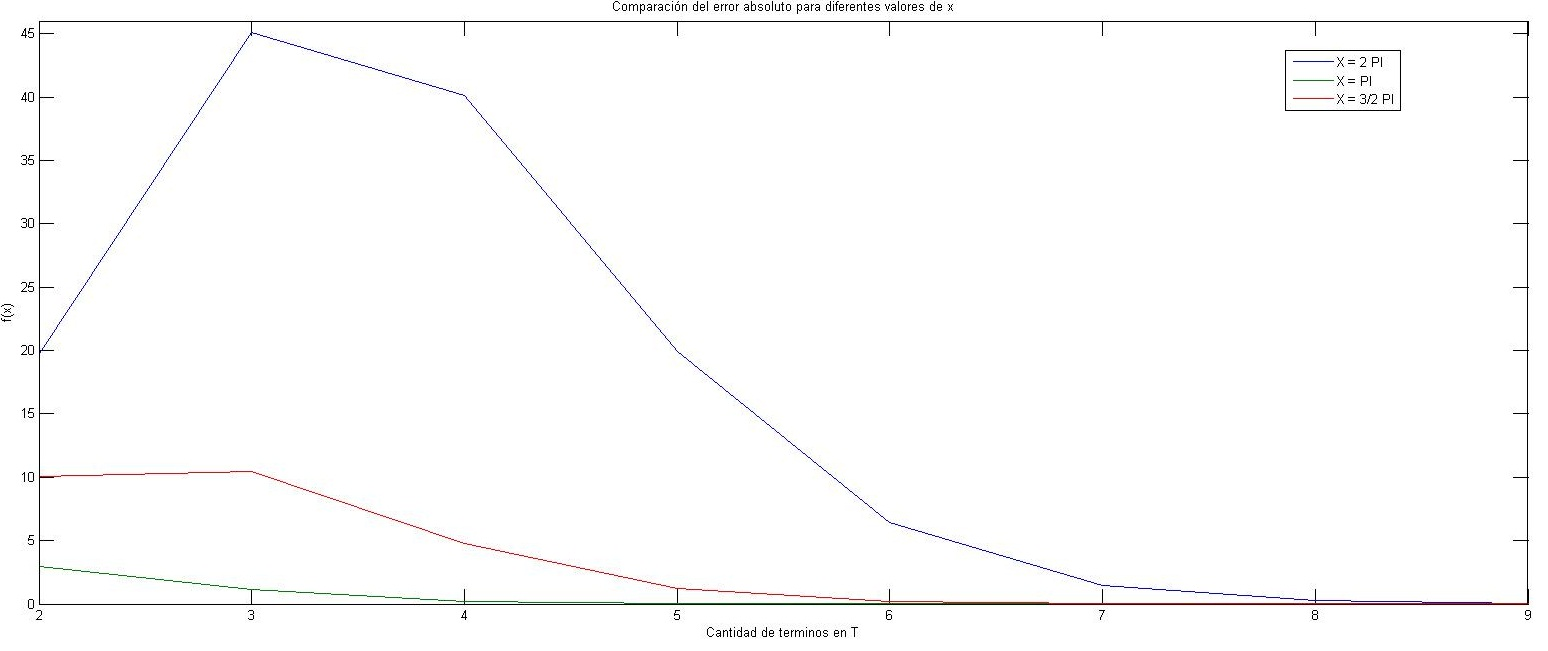
\includegraphics[scale=0.45]{../img/2a-xmayorPI.jpg} \\
 	\scriptsize{\textsf{\textbf{Gr\'afico 2.2, comparación del error absoluto para diferentes entradas $x$}}}
 	
\end{center}

\subsubsection{Comportamiento de la función para una cantidad de términos fija y un espectro de entrada más grande}


Seguidamente quisimos analizar el comportamiento para un T más grande, para esto tomamos T=10 y comparamos los resultados obtenidos entre $f(x)$ y $cos(x)$ para valores entre 0 y 10

\begin{center}

	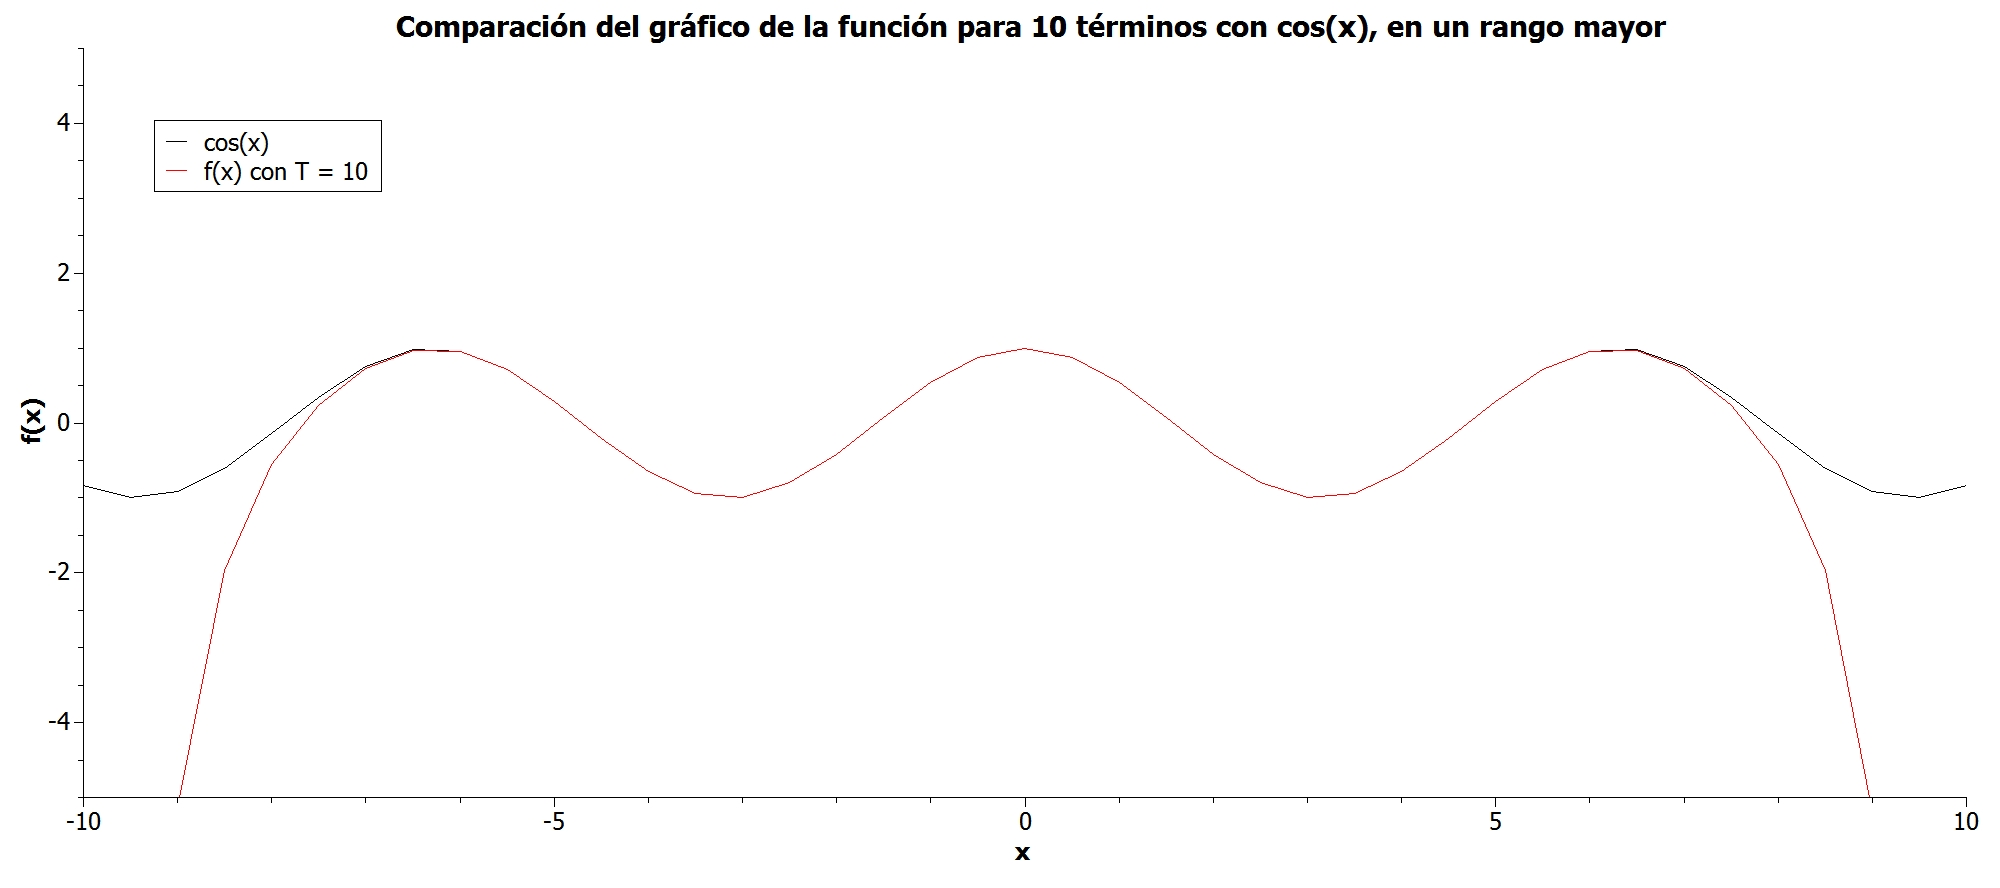
\includegraphics[scale=0.35]{../img/2afijo.jpg} \\
 	\scriptsize{\textsf{\textbf{Gr\'afico 1.3, comparación de $f(x)$ con un número de términos fijo = 10 contra la curva $\cos (x)$, para un rango mayor de números}}}
 	
\end{center}

\subsection{Análisis con tamaños de mantisa variable}

Para esta sección, comparamos el comportamiento de la aproximación en función de la cantidad de términos, de la entrada y del tamaño de la mantisa elegida

\subsubsection{Comparación del comportamiento en función de la cantidad de términos}

En primer lugar, decidimos observar el comportamiento en función de la cantidad de términos, para esto, elegimos tres entradas $x$, como ser $\pi$, $2\pi$ y $\3pi$ y tres tamaños de mantisa diferentes, 2, 15 y 50

\begin{center}
	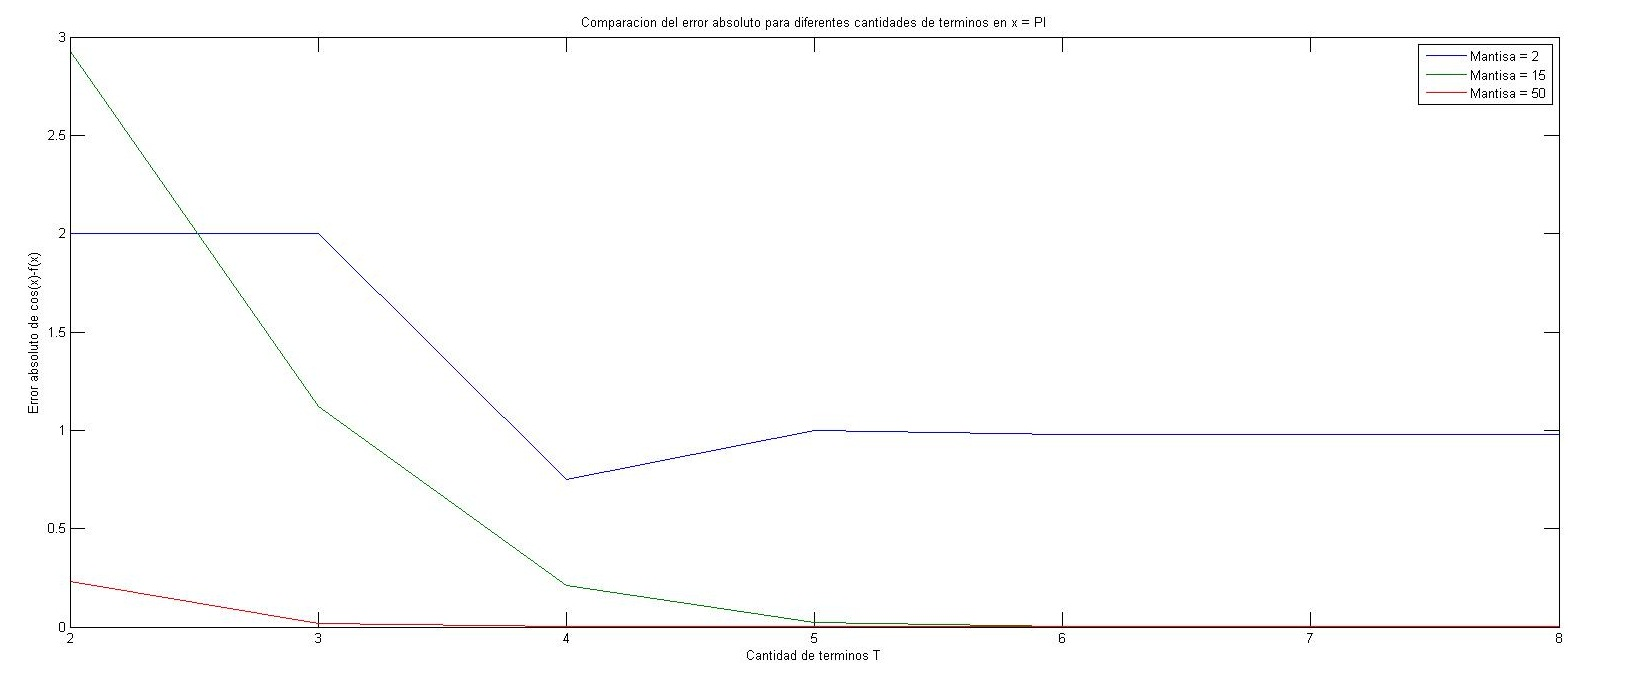
\includegraphics[scale=0.45]{../img/2b-term-pi.jpg} \\
 	\scriptsize{\textsf{\textbf{Gr\'afico 3.1, comparación del error absoluto para diferentes cantidades de términos, con x=$\pi$ y tres tamaños de mantisa diferentes}}}
 	
\end{center}

\begin{center}
	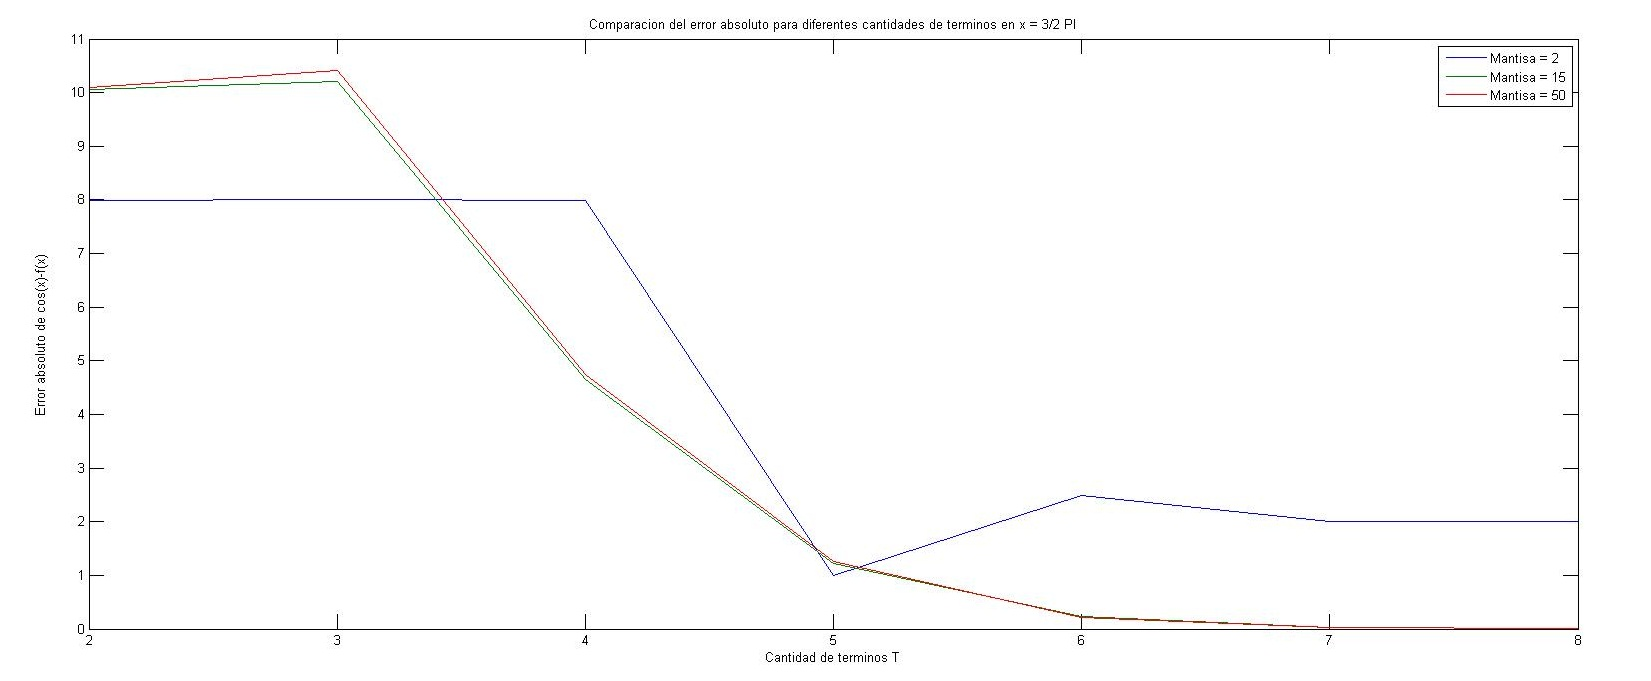
\includegraphics[scale=0.45]{../img/2b-term-32pi.jpg} \\
 	\scriptsize{\textsf{\textbf{Gr\'afico 3.2, comparación del error absoluto para diferentes cantidades de términos, con x=$\frac{3}{2}\pi$ y tres tamaños de mantisa diferentes}}}
 	
\end{center}

\begin{center}
	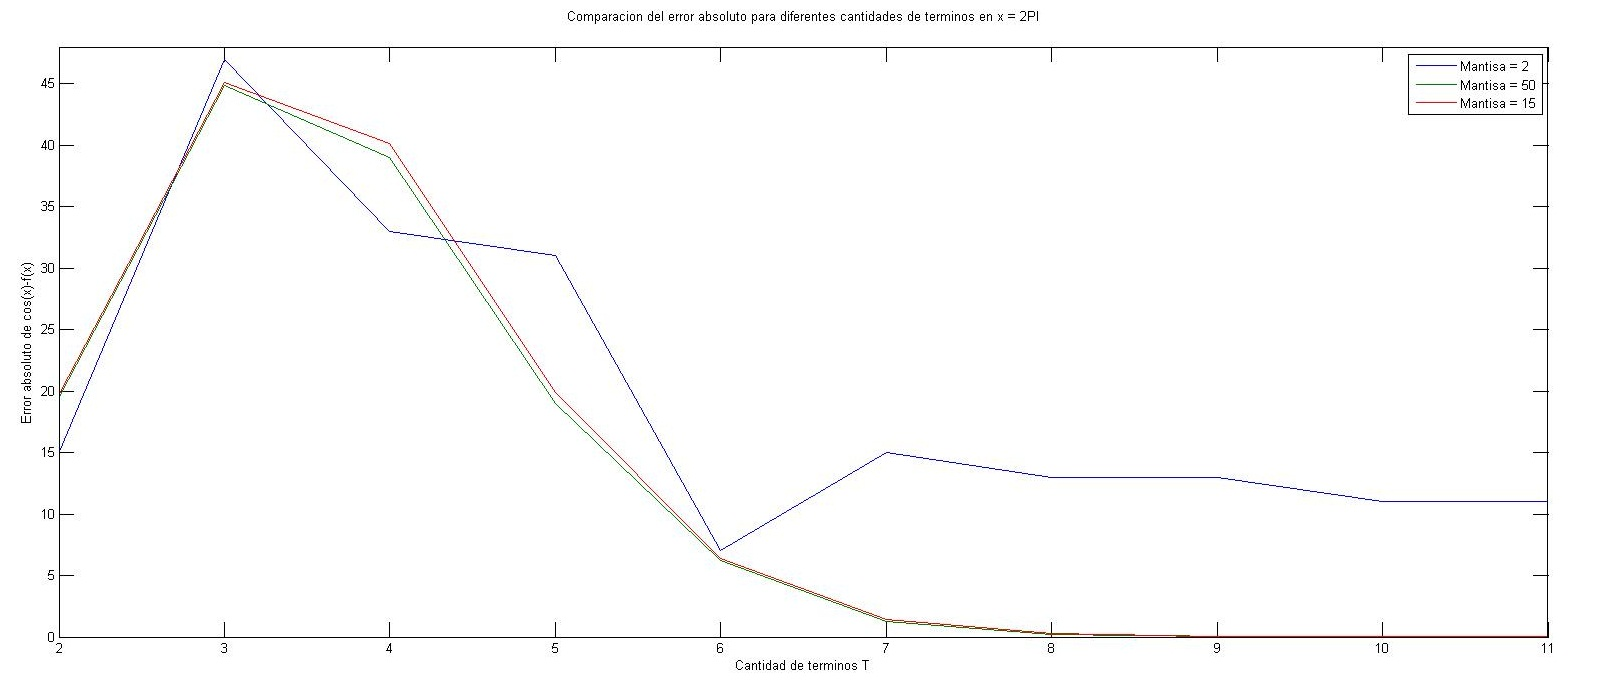
\includegraphics[scale=0.45]{../img/2b-term-2pi.jpg} \\
 	\scriptsize{\textsf{\textbf{Gr\'afico 3.3, comparación del error absoluto para diferentes cantidades de términos, con x=$2\pi$ y tres tamaños de mantisa diferentes}}}
 	
\end{center}



\subsubsection{Comparación del comportamiento en función del tamaño de la mantisa}

Luego estudiamos el comportamiento en función del tamaño de la mantisa, para esto, elegimos tres entradas $x$, como ser $\frac{1}{2}\pi$, $\pi$, y $\frac{3}{2}\pi$ y tres cantidades de términos diferentes, 2, 4 y 6


\begin{center}
	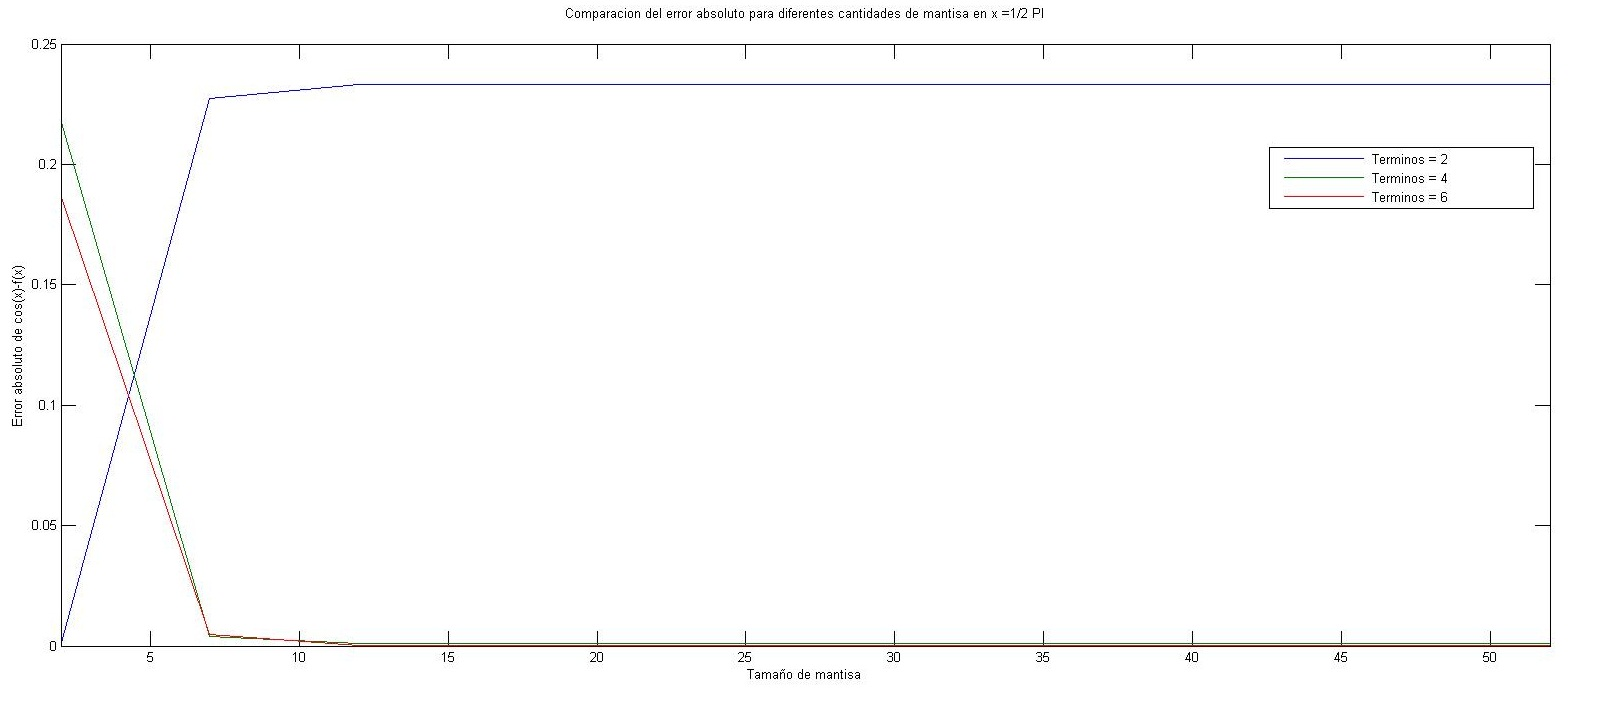
\includegraphics[scale=0.45]{../img/2b-mant-12pi.jpg} \\
 	\scriptsize{\textsf{\textbf{Gr\'afico 4.1, comparación del error absoluto para diferentes tamaños de mantisa, con x=$\frac{1}{2}\pi$ y tres cantidades de términos diferentes}}}
 	
\end{center}

\begin{center}
	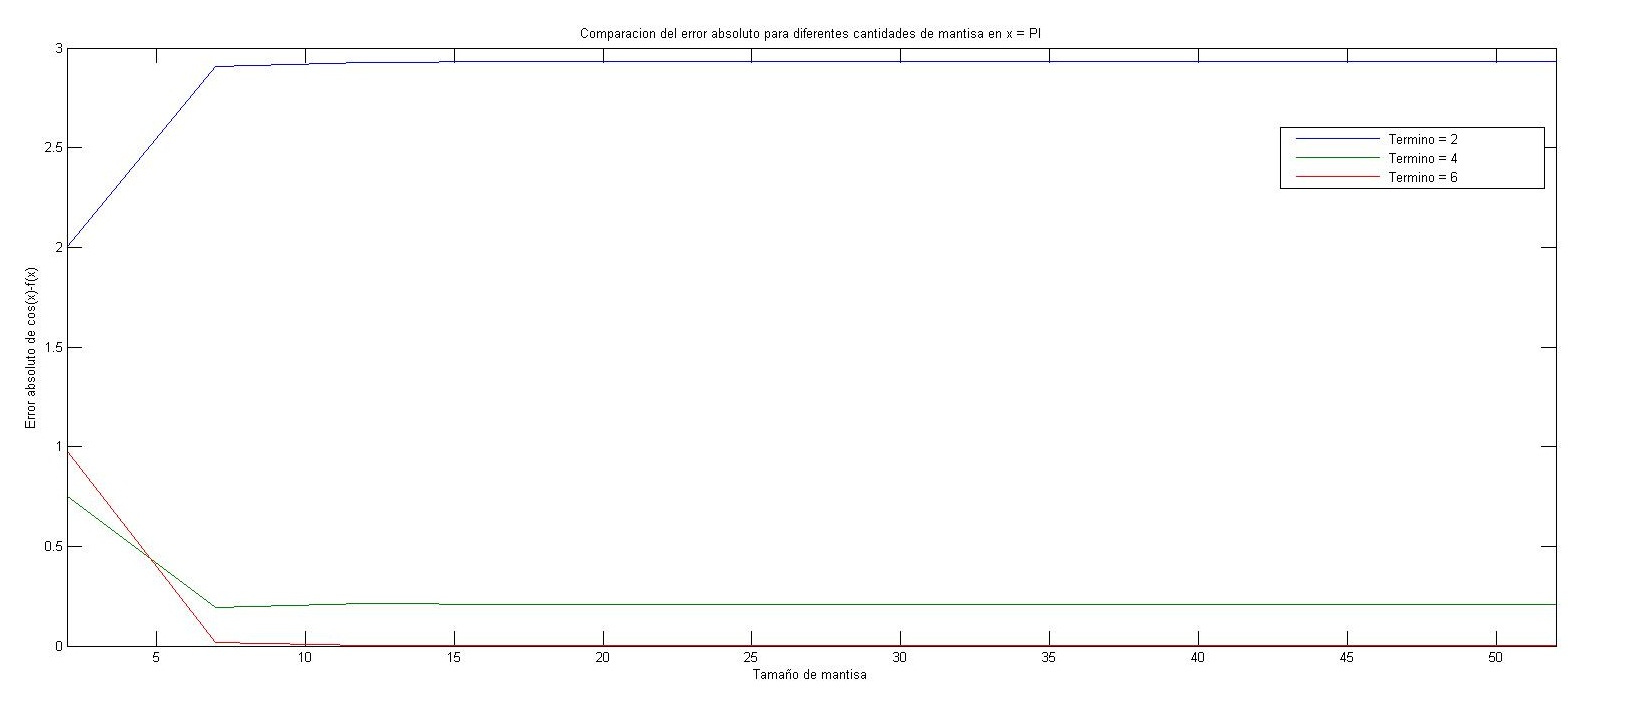
\includegraphics[scale=0.45]{../img/2b-mant-pi.jpg} \\
 	\scriptsize{\textsf{\textbf{Gr\'afico 4.2, comparación del error absoluto para diferentes tamaños de mantisa, con x=$\pi$ y tres cantidades de términos diferentes}}}
 	
\end{center}

\begin{center}
	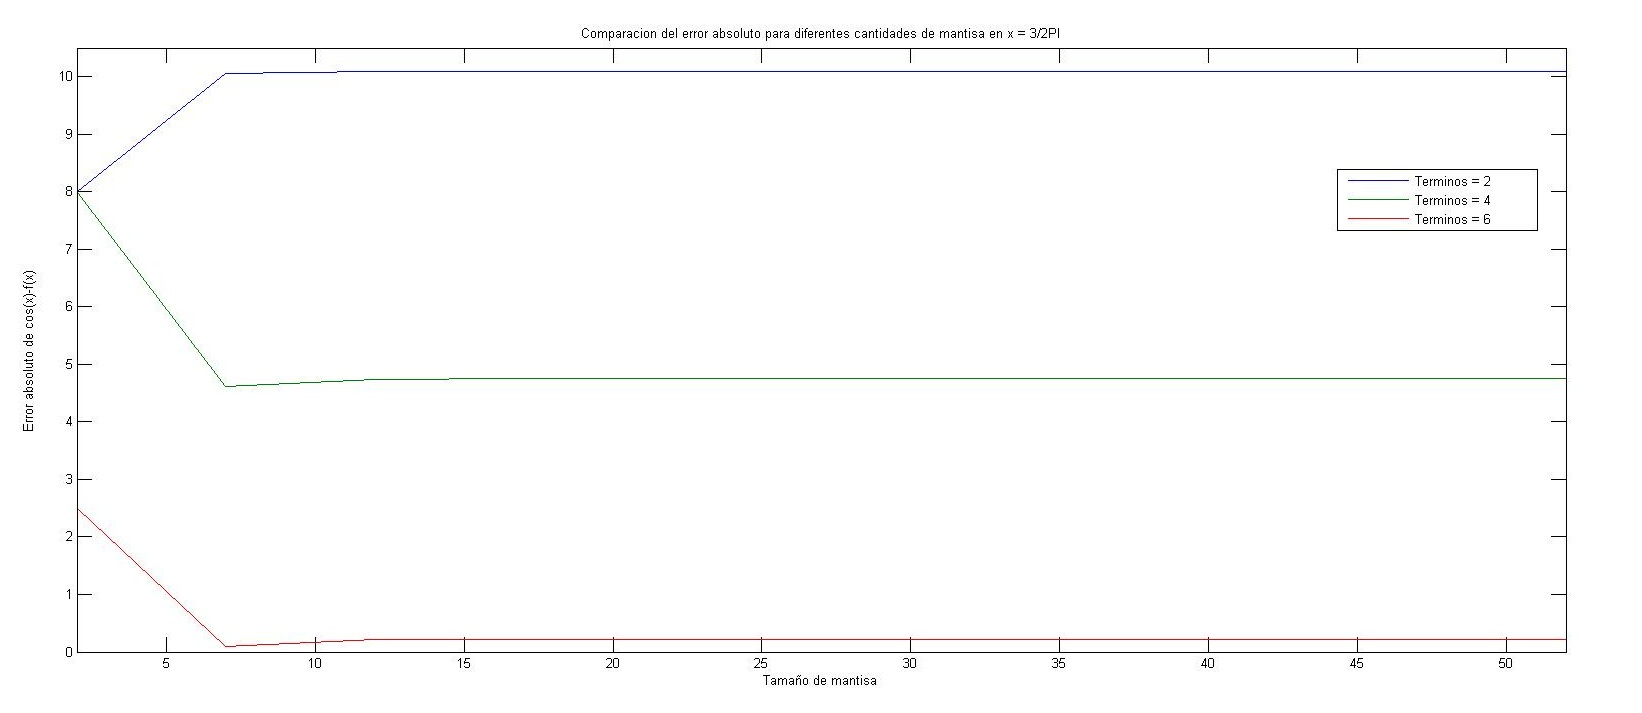
\includegraphics[scale=0.45]{../img/2b-mant-32pi.jpg} \\
 	\scriptsize{\textsf{\textbf{Gr\'afico 4.3, comparación del error absoluto para diferentes tamaños de mantisa, con x=$\frac{3}{2}\pi$ y tres cantidades de términos diferentes}}}
 	
\end{center}

\subsubsection{Comparación del comportamiento en función del valor de la entrada}

También analizamos el comportamiento en función del valor de la entrada, para esto, elegimos tres cantidades de términos diferentes, 2, 4 y 6 y tres tamaños de mantisa diferentes, 2, 15 y 50

\begin{center}
	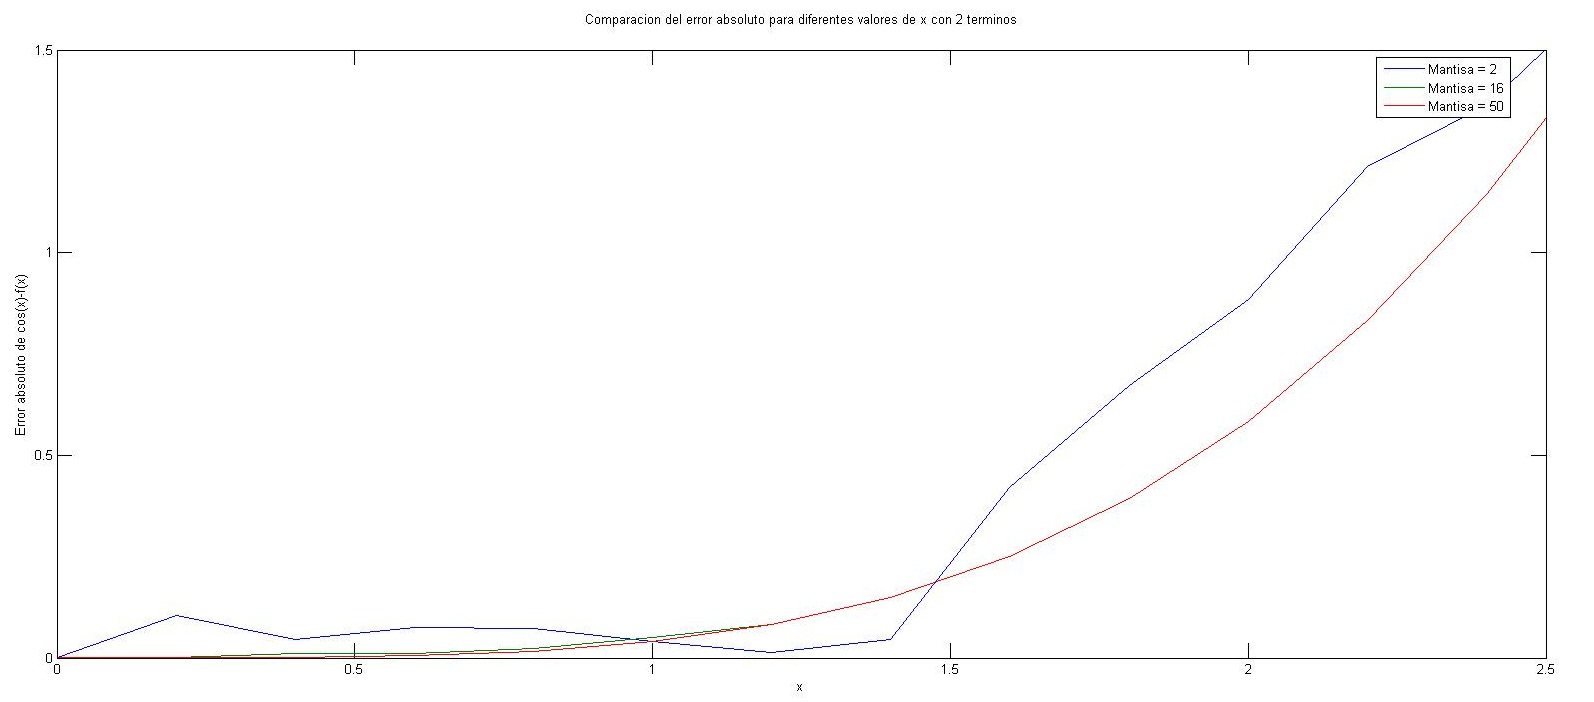
\includegraphics[scale=0.45]{../img/2b-x-2t.jpg} \\
 	\scriptsize{\textsf{\textbf{Gr\'afico 5.1, comparación del error absoluto para diferentes entradas, con T=2 y tres tamaños de mantisa diferentes}}}
 	
\end{center}

\begin{center}
	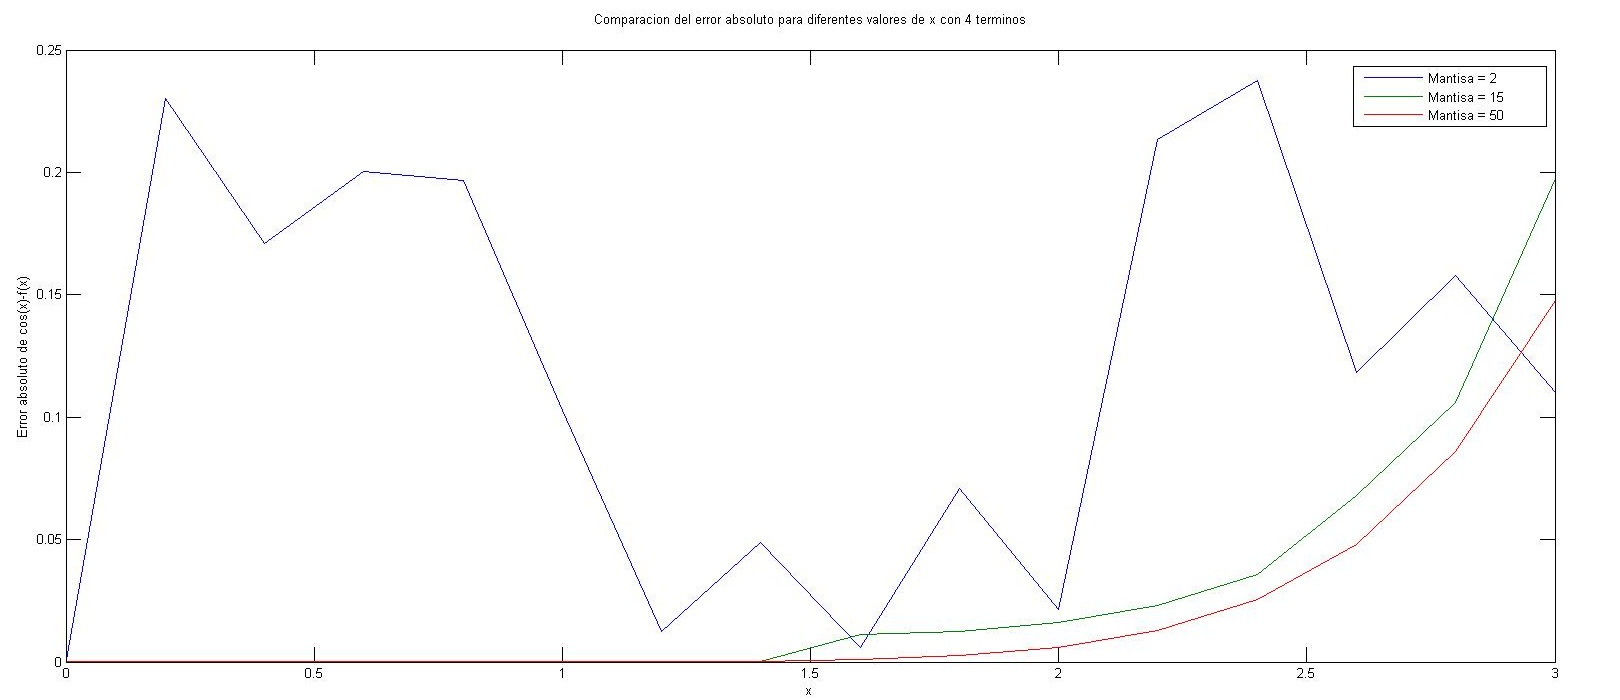
\includegraphics[scale=0.45]{../img/2b-x-4t.jpg} \\
 	\scriptsize{\textsf{\textbf{Gr\'afico 5.2, comparación del error absoluto para diferentes entradas, con T=4 y tres tamaños de mantisa diferentes}}}
 	
\end{center}

\begin{center}
	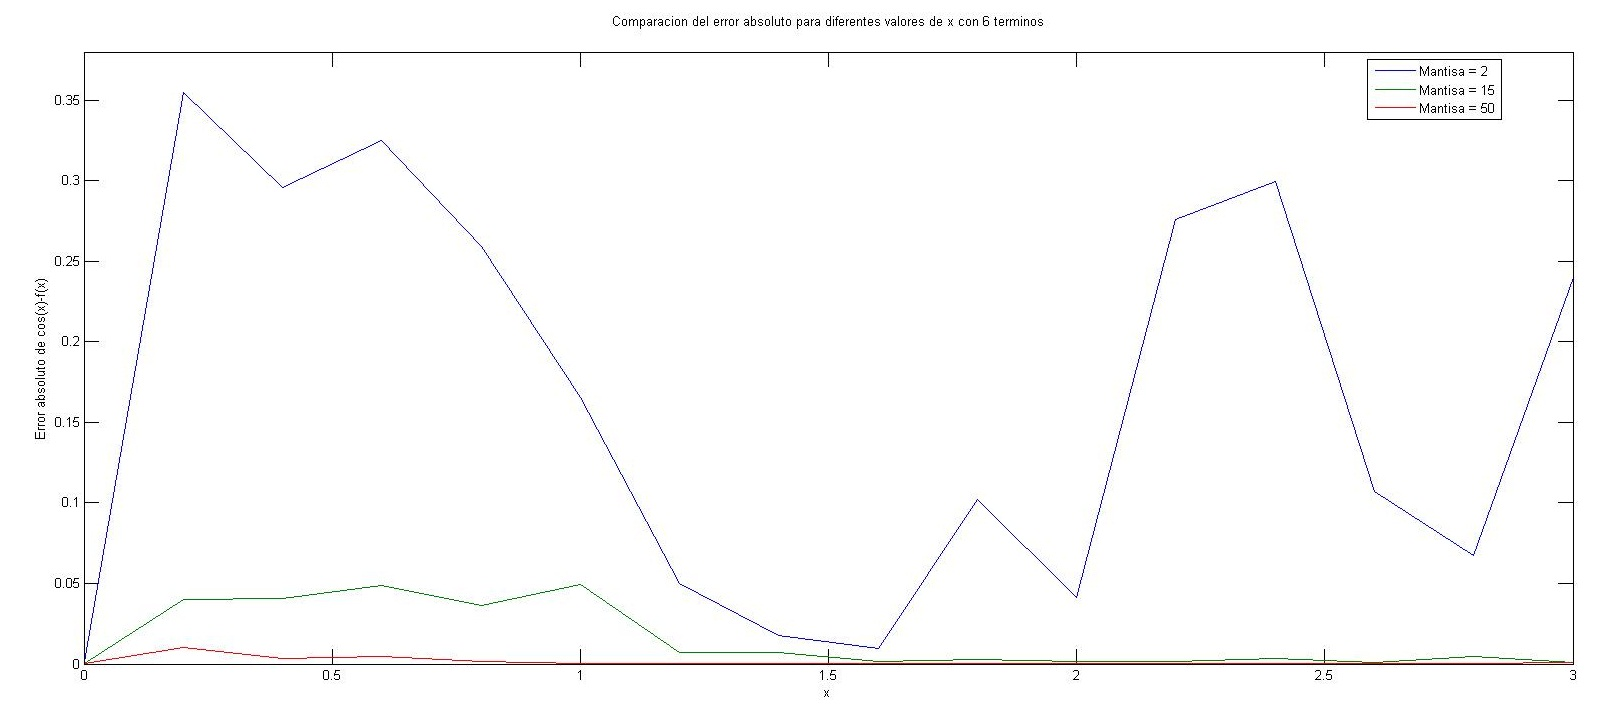
\includegraphics[scale=0.45]{../img/2b-x-6t.jpg} \\
 	\scriptsize{\textsf{\textbf{Gr\'afico 5.3, comparación del error absoluto para diferentes entradas, con T=6 y tres tamaños de mantisa diferentes}}}
 	
\end{center}

\vspace{1cm}

\subsubsection{Comparación de errores obtenidos por la sumatoria con los teóricos}

Finalmente analizamos como el error teórico hace una curva similar a la curva dada por el error que produce nuestro algorítmo usando un $x$ fijo ($x=2,4$) y variando la cantidad de términos utilizados de la serie de McLaurin. 

\begin{center}

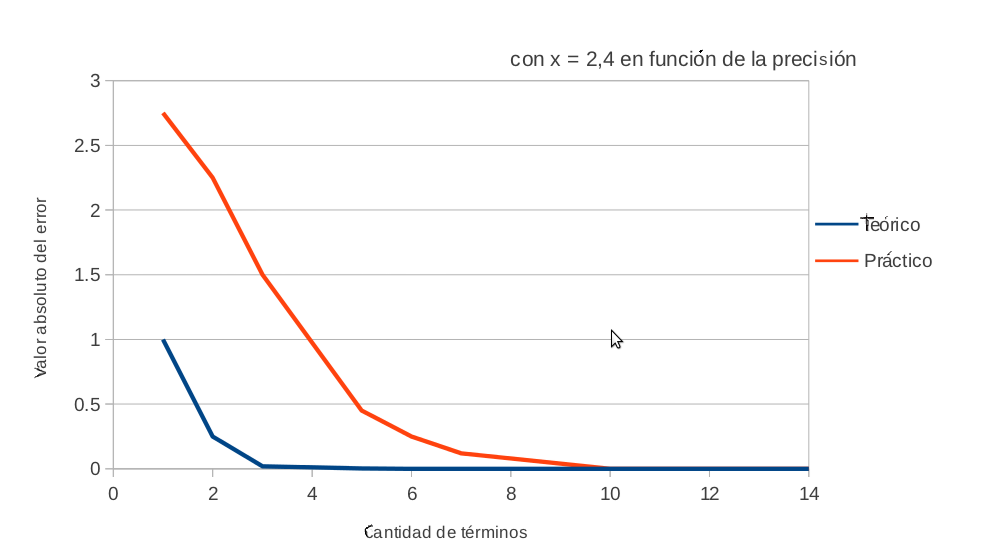
\includegraphics[scale=0.50]{../img/teorico.png} \\
\scriptsize{\textsf{\textbf{Gráfico 6.1, comparación de errores teóricos con los errores prácticos a medida que aumenta la cantidad de términos utilizados}}}

\end{center}
